\documentclass[11pt]{article}

\usepackage[margin=0.9in]{geometry}
\usepackage[T1]{fontenc}
\usepackage[utf8]{inputenc}
\usepackage{lmodern}
\usepackage{booktabs}
\usepackage{array}
\usepackage{siunitx}
\usepackage{amsmath}
\usepackage{tikz}
\usepackage{pgfplots}
\usepackage{subcaption}
\usepackage{xcolor}
\usepackage{hyperref}
\usepackage{enumitem}

\pgfplotsset{compat=1.18}
\sisetup{detect-all}

\definecolor{vcyan}{HTML}{00E5FF}
\definecolor{vgreen}{HTML}{76FF03}
\definecolor{vorange}{HTML}{FF9100}
\definecolor{vmagenta}{HTML}{D500F9}

\pgfplotsset{
  darkaxis/.style={
    width=\linewidth,
    height=5.5cm,
    axis background/.style={fill=black},
    grid=both,
    grid style={draw=gray!45},
    major grid style={draw=gray!55},
    axis line style={white},
    tick style={white},
    ticklabel style={color=white,font=\scriptsize},
    label style={color=white,font=\small},
    title style={color=white,font=\small\bfseries},
    legend style={draw=none, fill=black, text=white, font=\scriptsize},
    line join=bevel
  }
}

\title{\textbf{NeuroCore Workthrough:}\\
Transistor-Level Neuromorphic Compute to GDSII Flow Evidence}
\author{Project Log Date: 2026-02-03}
\date{}

\begin{document}
\maketitle

\begin{abstract}
This workthrough documents a reproducible hardware-development path built in one repository:
(1) analog neuromorphic circuits verified at transistor level in Spectre/OCEAN,
(2) a completed digital stack from CMOS primitives to GPU-core-level hierarchy, and
(3) a script-driven implementation smoke flow that reaches routed physical artifacts and GDSII output.
Unlike polished concept slides, the figures in this report are plotted directly from sampled electrical data points (no smoothing) with a dark-scope visual style for video-aligned evidence presentation.
\end{abstract}

\section{Project Snapshot}

\begin{table}[h]
\centering
\caption{Current execution status (competition-facing view).}
\begin{tabular}{>{\raggedright\arraybackslash}p{4.0cm} >{\raggedright\arraybackslash}p{2.0cm} >{\raggedright\arraybackslash}p{6.7cm}}
\toprule
\textbf{Track} & \textbf{Status} & \textbf{Evidence} \\
\midrule
Analog path (\texttt{synapse} \textrightarrow{} \texttt{neuro\_tile4\_coupled}) & PASS &
\texttt{competition/verification-evidence.md} \\
Digital hierarchy (CMOS \textrightarrow{} GPU core) & PASS &
\texttt{results/gpu\_core\_test.txt} \\
Robustness sweep (63-point matrix) & PASS (63/63) &
\texttt{competition/paper/data/neuro\_tile4\_coupled\_sweep\_parsed.csv} \\
Synopsys DC smoke & BLOCKED (license) &
\texttt{implementation/fullflow\_demo/work/dc/reports/alu4\_flow\_demo\_dc\_fallback.warn} \\
Cadence Innovus smoke & PASS &
\texttt{implementation/fullflow\_demo/work/innovus/out/alu4\_flow\_demo.gds} \\
Siemens Calibre smoke & BLOCKED (license) &
\texttt{implementation/fullflow\_demo/work/calibre/alu4\_flow\_demo\_drc.summary} \\
\bottomrule
\end{tabular}
\label{tab:status}
\end{table}

\begin{figure}[h]
\centering
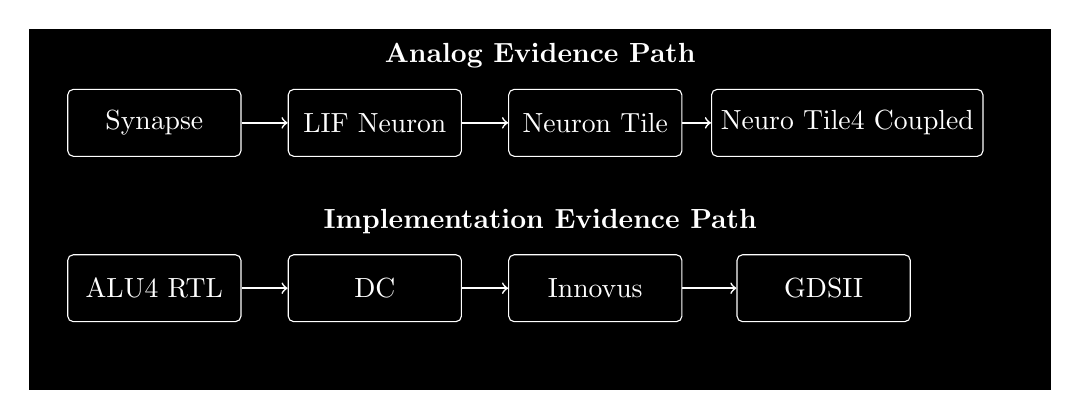
\begin{tikzpicture}[x=1cm,y=1cm]
  \fill[black] (0,0) rectangle (13,4.6);
  \draw[white, line width=0.5pt] (0,0) rectangle (13,4.6);

  \node[draw=white, rounded corners=2pt, fill=black, text=white, minimum width=2.2cm, minimum height=0.85cm] (a1) at (1.6,3.4) {Synapse};
  \node[draw=white, rounded corners=2pt, fill=black, text=white, minimum width=2.2cm, minimum height=0.85cm] (a2) at (4.4,3.4) {LIF Neuron};
  \node[draw=white, rounded corners=2pt, fill=black, text=white, minimum width=2.2cm, minimum height=0.85cm] (a3) at (7.2,3.4) {Neuron Tile};
  \node[draw=white, rounded corners=2pt, fill=black, text=white, minimum width=2.6cm, minimum height=0.85cm] (a4) at (10.4,3.4) {Neuro Tile4 Coupled};

  \node[draw=white, rounded corners=2pt, fill=black, text=white, minimum width=2.2cm, minimum height=0.85cm] (d1) at (1.6,1.3) {ALU4 RTL};
  \node[draw=white, rounded corners=2pt, fill=black, text=white, minimum width=2.2cm, minimum height=0.85cm] (d2) at (4.4,1.3) {DC};
  \node[draw=white, rounded corners=2pt, fill=black, text=white, minimum width=2.2cm, minimum height=0.85cm] (d3) at (7.2,1.3) {Innovus};
  \node[draw=white, rounded corners=2pt, fill=black, text=white, minimum width=2.2cm, minimum height=0.85cm] (d4) at (10.1,1.3) {GDSII};

  \draw[->,white,line width=0.6pt] (a1) -- (a2);
  \draw[->,white,line width=0.6pt] (a2) -- (a3);
  \draw[->,white,line width=0.6pt] (a3) -- (a4);
  \draw[->,white,line width=0.6pt] (d1) -- (d2);
  \draw[->,white,line width=0.6pt] (d2) -- (d3);
  \draw[->,white,line width=0.6pt] (d3) -- (d4);

  \node[text=white, font=\bfseries] at (6.5,4.25) {Analog Evidence Path};
  \node[text=white, font=\bfseries] at (6.5,2.15) {Implementation Evidence Path};
\end{tikzpicture}
\caption{End-to-end evidence structure used in the demo narrative.}
\label{fig:stack-diagram}
\end{figure}

\section{Architecture Dissection and Compute Model}

This work uses a bottom-up analog composition path:
\texttt{synapse} \textrightarrow{} \texttt{lif\_neuron} \textrightarrow{} \texttt{neuron\_tile}
\textrightarrow{} \texttt{neuro\_tile4} \textrightarrow{} \texttt{neuro\_tile4\_coupled}
\textrightarrow{} \texttt{neuro\_tile4\_mixed\_signal}.
The architecture note for paper drafting is maintained at
\texttt{competition/paper/architecture-dissection.md}.

Dissection protocol in this workthrough is intentionally systematic:
\textbf{(1)} structure pass, \textbf{(2)} dynamics pass, \textbf{(3)} evidence pass.
Each paper claim is tied to an explicit artifact path so the narrative remains auditable.
The full "draw-everything" component atlas is maintained at
\texttt{competition/paper/full-architecture-atlas.md}.

\begin{figure}[h]
\centering
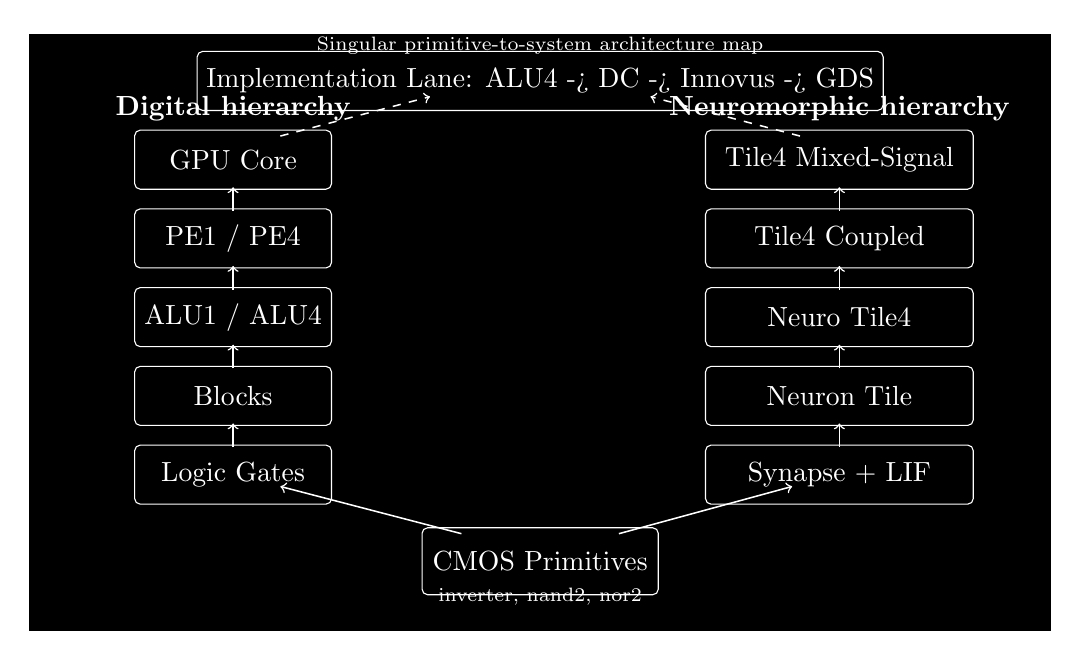
\begin{tikzpicture}[x=1cm,y=1cm]
  \fill[black] (0,0) rectangle (13,7.6);
  \draw[white, line width=0.5pt] (0,0) rectangle (13,7.6);

  % Root primitives
  \node[draw=white, rounded corners=2pt, fill=black, text=white, minimum width=3.0cm, minimum height=0.85cm] (p0) at (6.5,0.9) {CMOS Primitives};
  \node[text=white, font=\scriptsize] at (6.5,0.45) {inverter, nand2, nor2};

  % Digital chain (left)
  \node[draw=white, rounded corners=2pt, fill=black, text=white, minimum width=2.5cm, minimum height=0.75cm] (d1) at (2.6,2.0) {Logic Gates};
  \node[draw=white, rounded corners=2pt, fill=black, text=white, minimum width=2.5cm, minimum height=0.75cm] (d2) at (2.6,3.0) {Blocks};
  \node[draw=white, rounded corners=2pt, fill=black, text=white, minimum width=2.5cm, minimum height=0.75cm] (d3) at (2.6,4.0) {ALU1 / ALU4};
  \node[draw=white, rounded corners=2pt, fill=black, text=white, minimum width=2.5cm, minimum height=0.75cm] (d4) at (2.6,5.0) {PE1 / PE4};
  \node[draw=white, rounded corners=2pt, fill=black, text=white, minimum width=2.5cm, minimum height=0.75cm] (d5) at (2.6,6.0) {GPU Core};

  % Analog chain (right)
  \node[draw=white, rounded corners=2pt, fill=black, text=white, minimum width=3.4cm, minimum height=0.75cm] (a1) at (10.3,2.0) {Synapse + LIF};
  \node[draw=white, rounded corners=2pt, fill=black, text=white, minimum width=3.4cm, minimum height=0.75cm] (a2) at (10.3,3.0) {Neuron Tile};
  \node[draw=white, rounded corners=2pt, fill=black, text=white, minimum width=3.4cm, minimum height=0.75cm] (a3) at (10.3,4.0) {Neuro Tile4};
  \node[draw=white, rounded corners=2pt, fill=black, text=white, minimum width=3.4cm, minimum height=0.75cm] (a4) at (10.3,5.0) {Tile4 Coupled};
  \node[draw=white, rounded corners=2pt, fill=black, text=white, minimum width=3.4cm, minimum height=0.75cm] (a5) at (10.3,6.0) {Tile4 Mixed-Signal};

  % Implementation lane
  \node[draw=white, rounded corners=2pt, fill=black, text=white, minimum width=3.8cm, minimum height=0.75cm] (i0) at (6.5,7.0) {Implementation Lane: ALU4 -> DC -> Innovus -> GDS};

  % Branching arrows
  \draw[->,white,line width=0.55pt] (5.5,1.25) -- (3.2,1.85);
  \draw[->,white,line width=0.55pt] (7.5,1.25) -- (9.7,1.85);

  % Digital arrows
  \draw[->,white,line width=0.55pt] (2.6,2.35) -- (2.6,2.65);
  \draw[->,white,line width=0.55pt] (2.6,3.35) -- (2.6,3.65);
  \draw[->,white,line width=0.55pt] (2.6,4.35) -- (2.6,4.65);
  \draw[->,white,line width=0.55pt] (2.6,5.35) -- (2.6,5.65);

  % Analog arrows
  \draw[->,white,line width=0.55pt] (10.3,2.35) -- (10.3,2.65);
  \draw[->,white,line width=0.55pt] (10.3,3.35) -- (10.3,3.65);
  \draw[->,white,line width=0.55pt] (10.3,4.35) -- (10.3,4.65);
  \draw[->,white,line width=0.55pt] (10.3,5.35) -- (10.3,5.65);

  % Link to implementation lane
  \draw[->,white,dashed,line width=0.55pt] (3.2,6.3) -- (5.1,6.8);
  \draw[->,white,dashed,line width=0.55pt] (9.8,6.3) -- (7.9,6.8);

  % Labels
  \node[text=white, font=\bfseries] at (2.6,6.65) {Digital hierarchy};
  \node[text=white, font=\bfseries] at (10.3,6.65) {Neuromorphic hierarchy};
  \node[text=white, font=\scriptsize] at (6.5,7.45) {Singular primitive-to-system architecture map};
\end{tikzpicture}
\caption{Singular informative architecture diagram: all major verified components grouped from primitive root to digital and neuromorphic branches.}
\label{fig:singular-unified-map}
\end{figure}

\begin{table}[h]
\centering
\caption{Component-by-component architecture breakdown.}
\begin{tabular}{>{\raggedright\arraybackslash}p{2.9cm} >{\raggedright\arraybackslash}p{4.1cm} >{\raggedright\arraybackslash}p{4.8cm}}
\toprule
\textbf{Block} & \textbf{Mechanism} & \textbf{Compute role} \\
\midrule
Synapse & Charge injection + RC decay on \texttt{post} node & Converts input pulse stream into analog postsynaptic trajectory \\
LIF neuron & Membrane RC integration + threshold inverter chain + reset NMOS & Converts trajectory crossing into spike events \\
Neuron tile & Synapse output resistively coupled into membrane node & End-to-end local channel: pulse \textrightarrow{} state \textrightarrow{} event \\
Neuro Tile4 & Four replicated channels with staggered drives & Encodes information in relative spike timing \\
Neuro Tile4 Coupled & Feed-forward channel-to-channel injection links & Demonstrates asynchronous event propagation without clocking \\
Neuro Tile4 Mixed-Signal & Digital \texttt{en} gates analog propagation transistors & Demonstrates digital control over analog compute path \\
\bottomrule
\end{tabular}
\label{tab:arch-breakdown}
\end{table}

\begin{figure}[h]
\centering
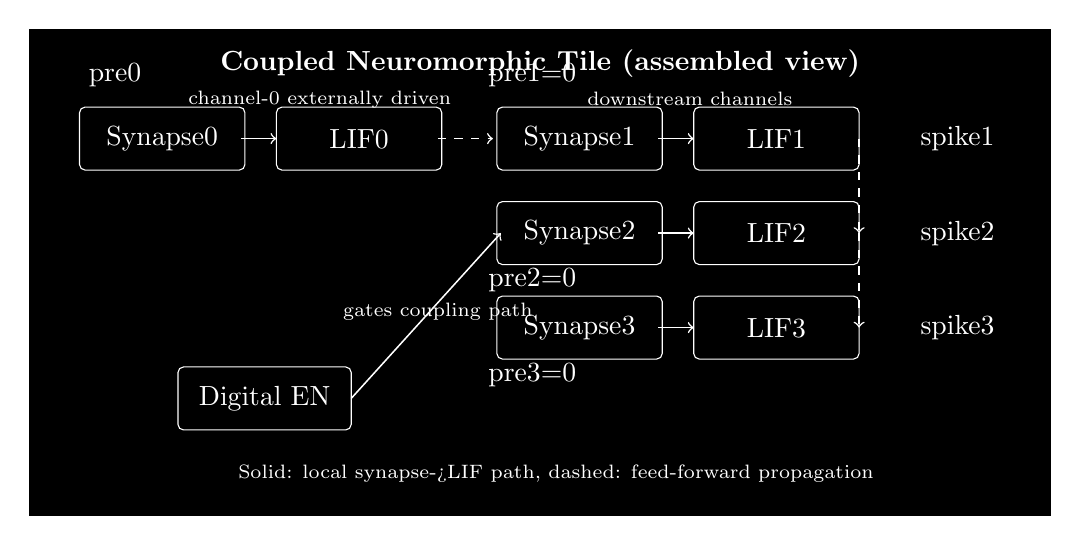
\begin{tikzpicture}[x=1cm,y=1cm]
  \fill[black] (0,0) rectangle (13,6.2);
  \draw[white, line width=0.5pt] (0,0) rectangle (13,6.2);

  % Analog core rail
  \node[draw=white, rounded corners=2pt, fill=black, text=white, minimum width=2.1cm, minimum height=0.8cm] (syn0) at (1.7,4.8) {Synapse0};
  \node[draw=white, rounded corners=2pt, fill=black, text=white, minimum width=2.1cm, minimum height=0.8cm] (lif0) at (4.2,4.8) {LIF0};
  \node[draw=white, rounded corners=2pt, fill=black, text=white, minimum width=2.1cm, minimum height=0.8cm] (syn1) at (7.0,4.8) {Synapse1};
  \node[draw=white, rounded corners=2pt, fill=black, text=white, minimum width=2.1cm, minimum height=0.8cm] (lif1) at (9.5,4.8) {LIF1};

  \node[draw=white, rounded corners=2pt, fill=black, text=white, minimum width=2.1cm, minimum height=0.8cm] (syn2) at (7.0,3.6) {Synapse2};
  \node[draw=white, rounded corners=2pt, fill=black, text=white, minimum width=2.1cm, minimum height=0.8cm] (lif2) at (9.5,3.6) {LIF2};
  \node[draw=white, rounded corners=2pt, fill=black, text=white, minimum width=2.1cm, minimum height=0.8cm] (syn3) at (7.0,2.4) {Synapse3};
  \node[draw=white, rounded corners=2pt, fill=black, text=white, minimum width=2.1cm, minimum height=0.8cm] (lif3) at (9.5,2.4) {LIF3};

  % Drive and outputs
  \node[text=white] at (1.1,5.6) {pre0};
  \node[text=white] at (6.4,5.6) {pre1=0};
  \node[text=white] at (6.4,3.0) {pre2=0};
  \node[text=white] at (6.4,1.8) {pre3=0};
  \node[text=white] at (11.8,4.8) {spike1};
  \node[text=white] at (11.8,3.6) {spike2};
  \node[text=white] at (11.8,2.4) {spike3};

  % Connections
  \draw[->,white,line width=0.55pt] (2.7,4.8) -- (3.15,4.8);
  \draw[->,white,line width=0.55pt] (8.0,4.8) -- (8.45,4.8);
  \draw[->,white,line width=0.55pt] (8.0,3.6) -- (8.45,3.6);
  \draw[->,white,line width=0.55pt] (8.0,2.4) -- (8.45,2.4);

  % Feed-forward coupling
  \draw[->,white,dashed,line width=0.55pt] (5.2,4.8) -- (5.9,4.8);
  \draw[->,white,dashed,line width=0.55pt] (10.55,4.8) -- (10.55,3.6);
  \draw[->,white,dashed,line width=0.55pt] (10.55,3.6) -- (10.55,2.4);

  % Enable control
  \node[draw=white, rounded corners=2pt, fill=black, text=white, minimum width=2.2cm, minimum height=0.8cm] (en) at (3.0,1.5) {Digital EN};
  \draw[->,white,line width=0.55pt] (4.1,1.5) -- (6.0,3.6);
  \node[text=white, font=\scriptsize] at (5.2,2.6) {gates coupling path};

  % Labels
  \node[text=white, font=\bfseries] at (6.5,5.75) {Coupled Neuromorphic Tile (assembled view)};
  \node[text=white, font=\scriptsize] at (3.7,5.3) {channel-0 externally driven};
  \node[text=white, font=\scriptsize] at (8.4,5.3) {downstream channels};
  \node[text=white, font=\scriptsize] at (6.7,0.55) {Solid: local synapse->LIF path, dashed: feed-forward propagation};
\end{tikzpicture}
\caption{Assembled architecture sketch used for paper reasoning: local analog channels, feed-forward coupling, and digital-enable gating.}
\label{fig:assembled-architecture}
\end{figure}

At model level, the dominant continuous-time behavior is captured by:
\begin{align}
\frac{dV_{\mathrm{post}}}{dt} &= \frac{I_{\mathrm{inj}}}{C_{\mathrm{post}}} - \frac{V_{\mathrm{post}}}{R_{\mathrm{decay}}C_{\mathrm{post}}} \\
C_{\mathrm{mem}}\frac{dV_{\mathrm{mem}}}{dt} &= I_{\mathrm{in}} - \frac{V_{\mathrm{mem}}}{R_{\mathrm{leak}}} - I_{\mathrm{reset}}(t)
\end{align}
with event condition \(V_{\mathrm{mem}} \ge V_{\mathrm{th}}\) producing a spike and
activating reset/coupling currents. In this framing, computation is carried by
trajectory shape and event timing, not only by synchronized logic state updates.

\begin{table}[h]
\centering
\caption{Claim-to-artifact traceability map (paper-critical claims only).}
\begin{tabular}{>{\raggedright\arraybackslash}p{5.5cm} >{\raggedright\arraybackslash}p{5.2cm}}
\toprule
\textbf{Claim} & \textbf{Artifact path} \\
\midrule
Synapse integrates and decays across repeated pulses & \texttt{results/synapse\_test.txt} \\
LIF neuron produces repeated threshold events & \texttt{results/lif\_neuron\_test.txt} \\
Four-channel temporal staggering is preserved & \texttt{results/neuro\_tile4\_test.txt} \\
Channel-0 drive propagates downstream through coupling & \texttt{results/neuro\_tile4\_coupled\_test.txt} \\
Digital enable gates analog propagation & \texttt{results/neuro\_tile4\_mixed\_signal\_test.txt} \\
Founder-math metrics (fit/sensitivity/energy) are reproducible & \texttt{competition/analysis/*.md} \\
\bottomrule
\end{tabular}
\label{tab:traceability}
\end{table}

\section{Raw Electrical Data (No Smoothing)}

Data provenance note:
plots are drawn from exported CSV files in \texttt{competition/data/}, while
pass/fail metrics come from OCEAN verification reports in \texttt{results/}.
This keeps both waveform-level transparency and regression-style checks.

\subsection{Synapse and Tile-Level Spiking}

\begin{figure}[h]
\centering
\begin{tikzpicture}
\begin{axis}[
  darkaxis,
  title={Synapse Waveforms (sampled points)},
  xlabel={Time (ns)},
  ylabel={Voltage (V)},
  xmin=0, xmax=120,
  ymin=0, ymax=1.8,
  legend pos=north east
]
  \addplot+[sharp plot, line width=0.35pt, mark=*, mark size=0.25pt, color=vcyan]
    table[x=time_ns,y=pre,col sep=comma]{../data/synapse_waveform.csv};
  \addplot+[sharp plot, line width=0.35pt, mark=*, mark size=0.25pt, color=vgreen]
    table[x=time_ns,y=post,col sep=comma]{../data/synapse_waveform.csv};
  \addplot+[sharp plot, line width=0.35pt, mark=*, mark size=0.25pt, color=vorange]
    table[x=time_ns,y=out,col sep=comma]{../data/synapse_waveform.csv};
  \legend{pre, post, out}
\end{axis}
\end{tikzpicture}
\caption{Synapse waveform traces plotted directly from sampled CSV points.}
\label{fig:synapse}
\end{figure}

\begin{figure}[h]
\centering
\begin{tikzpicture}
\begin{axis}[
  darkaxis,
  title={Neuro Tile4 Spike Channels (raw points)},
  xlabel={Time (ns)},
  ylabel={Spike Voltage (V)},
  xmin=0, xmax=120,
  ymin=0, ymax=0.85,
  legend pos=north west
]
  \addplot+[sharp plot, line width=0.35pt, mark=*, mark size=0.22pt, color=vcyan]
    table[x=time_ns,y=spike0,col sep=comma]{../data/neuro_tile4_spikes.csv};
  \addplot+[sharp plot, line width=0.35pt, mark=*, mark size=0.22pt, color=vgreen]
    table[x=time_ns,y=spike1,col sep=comma]{../data/neuro_tile4_spikes.csv};
  \addplot+[sharp plot, line width=0.35pt, mark=*, mark size=0.22pt, color=vorange]
    table[x=time_ns,y=spike2,col sep=comma]{../data/neuro_tile4_spikes.csv};
  \addplot+[sharp plot, line width=0.35pt, mark=*, mark size=0.22pt, color=vmagenta]
    table[x=time_ns,y=spike3,col sep=comma]{../data/neuro_tile4_spikes.csv};
  \legend{spike0, spike1, spike2, spike3}
\end{axis}
\end{tikzpicture}
\caption{Four-channel spiking behavior showing preserved first-spike staggering across channels.}
\label{fig:tile4-spikes}
\end{figure}

\begin{figure}[h]
\centering
\begin{subfigure}[t]{0.49\linewidth}
\centering
\begin{tikzpicture}
\begin{axis}[
  darkaxis,
  title={Coupled Tile Spikes},
  xlabel={Time (ns)},
  ylabel={Voltage (V)},
  xmin=0, xmax=120,
  ymin=0, ymax=1.9,
  legend pos=north west
]
  \addplot+[sharp plot, line width=0.30pt, mark=*, mark size=0.20pt, color=vcyan]
    table[x=time_ns,y=spike0,col sep=comma]{../data/neuro_tile4_coupled_spikes.csv};
  \addplot+[sharp plot, line width=0.30pt, mark=*, mark size=0.20pt, color=vgreen]
    table[x=time_ns,y=spike1,col sep=comma]{../data/neuro_tile4_coupled_spikes.csv};
  \addplot+[sharp plot, line width=0.30pt, mark=*, mark size=0.20pt, color=vorange]
    table[x=time_ns,y=spike2,col sep=comma]{../data/neuro_tile4_coupled_spikes.csv};
  \addplot+[sharp plot, line width=0.30pt, mark=*, mark size=0.20pt, color=vmagenta]
    table[x=time_ns,y=spike3,col sep=comma]{../data/neuro_tile4_coupled_spikes.csv};
\end{axis}
\end{tikzpicture}
\end{subfigure}
\hfill
\begin{subfigure}[t]{0.49\linewidth}
\centering
\begin{tikzpicture}
\begin{axis}[
  darkaxis,
  title={Coupled Tile Membranes},
  xlabel={Time (ns)},
  ylabel={Voltage (V)},
  xmin=0, xmax=120,
  ymin=0, ymax=1.4,
  legend pos=north west
]
  \addplot+[sharp plot, line width=0.30pt, mark=*, mark size=0.20pt, color=vcyan]
    table[x=time_ns,y=mem0,col sep=comma]{../data/neuro_tile4_coupled_mems.csv};
  \addplot+[sharp plot, line width=0.30pt, mark=*, mark size=0.20pt, color=vgreen]
    table[x=time_ns,y=mem1,col sep=comma]{../data/neuro_tile4_coupled_mems.csv};
  \addplot+[sharp plot, line width=0.30pt, mark=*, mark size=0.20pt, color=vorange]
    table[x=time_ns,y=mem2,col sep=comma]{../data/neuro_tile4_coupled_mems.csv};
  \addplot+[sharp plot, line width=0.30pt, mark=*, mark size=0.20pt, color=vmagenta]
    table[x=time_ns,y=mem3,col sep=comma]{../data/neuro_tile4_coupled_mems.csv};
\end{axis}
\end{tikzpicture}
\end{subfigure}
\caption{Coupled-tile feed-forward propagation traces from sampled electrical data points.}
\label{fig:coupled-traces}
\end{figure}

\begin{table}[h]
\centering
\caption{Selected analog metrics from current verification reports (\texttt{results/*\_test.txt}).}
\begin{tabular}{lll}
\toprule
\textbf{Block} & \textbf{Metric} & \textbf{Value} \\
\midrule
Synapse & \(V_{\text{post,max}}\) & \SI{1.575}{V} \\
Synapse & Output pulse count & 6 \\
LIF neuron & Total spikes detected & 10 \\
LIF neuron & \(V_{\text{mem,max}}\) & \SI{1.573}{V} \\
Neuron tile & Spike-node pulses & 12 \\
Neuro Tile4 & First spike times & 27.5, 29.5, 31.5, 33.5 ns \\
Neuro Tile4 Coupled & Membrane maxima & 0.569, 0.974, 1.268, 0.873 V \\
Neuro Tile4 Coupled & Spike counts & 15, 15, 1, 1 \\
Neuro Tile4 Mixed-Signal & Downstream counts pre/post \texttt{en} & 0 \textrightarrow{} 7 per channel \\
\bottomrule
\end{tabular}
\label{tab:analog-metrics}
\end{table}

\section{Robustness Sweep Evidence}

\begin{figure}[h]
\centering
\begin{tikzpicture}
\begin{axis}[
  darkaxis,
  title={Sweep: Membrane Channel-2 Peak vs \(r_{fb}\)},
  xlabel={\(r_{fb}\) (Ohm)},
  ylabel={\(V_{\text{mem2,max}}\) (V)},
  xmin=650, xmax=1550,
  ymin=1.20, ymax=1.31,
  legend pos=south west
]
  \addplot+[sharp plot, mark=*, mark size=1.4pt, line width=0.6pt, color=vcyan]
    table[x=r_fb_ohm,y=mem2_max_v,col sep=comma]{data/sweep_mem2_rleak_6000000.csv};
  \addplot+[sharp plot, mark=square*, mark size=1.3pt, line width=0.6pt, color=vgreen]
    table[x=r_fb_ohm,y=mem2_max_v,col sep=comma]{data/sweep_mem2_rleak_8000000.csv};
  \addplot+[sharp plot, mark=triangle*, mark size=1.4pt, line width=0.6pt, color=vorange]
    table[x=r_fb_ohm,y=mem2_max_v,col sep=comma]{data/sweep_mem2_rleak_10000000.csv};
  \legend{\(r_{leak}=6\,\text{M}\Omega\), \(r_{leak}=8\,\text{M}\Omega\), \(r_{leak}=10\,\text{M}\Omega\)}
\end{axis}
\end{tikzpicture}
\caption{Sweep subset view (\(r_{leak}=6,8,10\)M\(\Omega\)) from parsed sweep CSV (\texttt{PASS}=63/63 total points).}
\label{fig:sweep}
\end{figure}

\begin{table}[h]
\centering
\caption{Sweep envelope summary from \texttt{neuro\_tile4\_coupled\_sweep\_parsed.csv}.}
\begin{tabular}{lcc}
\toprule
\textbf{Metric} & \textbf{Minimum} & \textbf{Maximum} \\
\midrule
\(V_{\text{mem0,max}}\) & 0.634 V & 0.647 V \\
\(V_{\text{mem1,max}}\) & 0.970 V & 1.012 V \\
\(V_{\text{mem2,max}}\) & 1.183 V & 1.244 V \\
\(V_{\text{mem3,max}}\) & 0.755 V & 0.757 V \\
Spike-count vector \((s0,s1,s2,s3)\) & \multicolumn{2}{c}{(15, 15, 15, 15) at all 63 points} \\
\bottomrule
\end{tabular}
\label{tab:sweep-envelope}
\end{table}

\section{Founder-Thesis Quantitative Evidence}

\begin{table}[h]
\centering
\caption{Math-oriented evidence tied to the continuous-time compute claim.}
\begin{tabular}{>{\raggedright\arraybackslash}p{4.0cm} >{\raggedright\arraybackslash}p{2.2cm} >{\raggedright\arraybackslash}p{6.4cm}}
\toprule
\textbf{Evidence track} & \textbf{Value} & \textbf{Artifact} \\
\midrule
LIF decay-window ODE fit \(R^2\) & 0.931 & \texttt{competition/analysis/lif\_ode\_fit\_summary.md} \\
Temporal sensitivity \(dt_{\text{spike0}}/dr_{fb}\) & -0.599 ns/kOhm (mean) & \texttt{competition/analysis/temporal\_sensitivity\_summary.md} \\
Energy per spike (first-pass estimate) & 4.718 pJ/spike & \texttt{competition/analysis/lif\_energy\_summary.md} \\
Mixed-signal gating check & pre-enable off, post-enable on & \texttt{competition/mixed-signal-smoke-evidence.md} \\
\bottomrule
\end{tabular}
\label{tab:founder-evidence}
\end{table}

\section{Implementation Flow Artifacts}

\begin{table}[h]
\centering
\caption{Full-flow smoke outputs for \texttt{alu4\_flow\_demo}.}
\begin{tabular}{>{\raggedright\arraybackslash}p{2.2cm} >{\raggedright\arraybackslash}p{1.8cm} >{\raggedright\arraybackslash}p{7.0cm}}
\toprule
\textbf{Stage} & \textbf{Result} & \textbf{Artifact(s)} \\
\midrule
DC & Blocked (license) & \texttt{dc\_shell.log}, fallback mapped netlist \\
Innovus & PASS & \texttt{alu4\_flow\_demo.def}, \texttt{alu4\_flow\_demo.gds}, post-route netlist \\
Calibre DRC & Blocked (license) & \texttt{alu4\_flow\_demo\_drc.summary} \\
\midrule
Area (Innovus) & --- & 10 instances, total area = 20.520 \\
Power (Innovus) & --- & total power = 0.00069651 mW \\
\bottomrule
\end{tabular}
\label{tab:fullflow}
\end{table}

\section{Reproducibility Commands}

\begin{itemize}[leftmargin=1.2em]
  \item Build and verify stack: \texttt{source setup\_cadence.sh} then \texttt{./build.sh all}
  \item Refresh competition visuals: \texttt{scripts/run\_competition\_visuals.sh}
  \item Parse paper helper data: \texttt{python3 scripts/prepare\_paper\_data.py}
  \item Full-flow smoke replay: \texttt{scripts/run\_fullflow\_smoke.sh}
  \item Strict mode (fail on blocked stages): \texttt{FULLFLOW\_STRICT=1 scripts/run\_fullflow\_smoke.sh}
\end{itemize}

\section{Current Limitations and Hardening Roadmap}

\begin{itemize}[leftmargin=1.2em]
  \item Full-window LIF ODE fit quality is weak relative to the decay-window fit, so model claims are bounded to validated regimes.
  \item Temporal-sensitivity sweep currently uses a coarse parameter grid; higher-resolution sweeps are tracked in \texttt{my-workspace/tickets/0013-evidence-rigor-hardening.md}.
  \item Full DC and Calibre closure remains license-blocked in this environment; reports are captured as explicit blocked-stage artifacts.
  \item Next hardening pass: denser sweep sampling, uncertainty bars on founder metrics, and release-grade evidence pack freeze.
\end{itemize}

\section{Conclusion}

This repository now demonstrates a practical and auditable path from transistor-level
analog neuromorphic behavior to physical implementation artifacts.
The key contribution for competition use is not a single benchmark number but a
repeatable engineering chain:
\textit{measured electrical traces, robustness sweeps, scripted implementation flow,
and concrete GDSII output artifacts}.
That combination is designed to be shown live in one terminal session and defended
with raw-source files.

\end{document}
